% Chapter 25 -- From Claim to Study: Research Design in Empirical Finance
% Requires: amsmath, amssymb, booktabs, array, tabularx, graphicx, tcolorbox (breakable, skins), hyperref or url.
% Defines the callout box only if the preamble has not.
\providecolor{fenavy}{HTML}{1B2A6B}
\providecolor{feshade}{HTML}{F3F5FA}
\makeatletter
\@ifundefined{callout}{%
  \newtcolorbox{callout}{breakable, enhanced,
    colback=white, colframe=gray!70, boxrule=0.5pt, arc=1mm,
    borderline west={2.5pt}{0pt}{gray!70},
    left=8pt, right=8pt, top=4pt, bottom=4pt}%
}{}
\makeatother

\chapter{From Claim to Study: Research Design in Empirical Finance}
\label{ch:25}

Chapters 7 to 24 put other people's claims on trial. This chapter and the next turn the reader into the one making claims. A replication or an original study is only as credible as its design, and most of the failures this book has documented were failures of design rather than of arithmetic:

\begin{itemize}
  \item samples too short to detect the effect claimed;
  \item many specifications tried and one reported;
  \item benchmarks chosen after the results were known;
  \item null results left in a drawer.
\end{itemize}

The remedies are well known in medicine and psychology, and finance has begun to adopt them. They are decided before the data are touched: a precise hypothesis, a sample and benchmark fixed in advance, a power calculation, a written plan and a commitment to report what was found.

By the end of the chapter you will be able to:

\begin{itemize}
  \item explain type I and type II errors, power and p-values, and compute the sample needed to detect a Sharpe ratio or a predictive $R^2$;
  \item adjust significance thresholds for multiple tests, and compute a Bayesianized p-value from a t-statistic and prior odds;
  \item describe the main tools of causal identification and the threats each addresses;
  \item turn a verbal claim into testable hypotheses with a primary test and a decision rule;
  \item choose a sample, benchmark and controls, and defend each choice;
  \item write and time-stamp a pre-registration;
  \item design a robustness grid and report it honestly, including null results;
  \item read a finance paper with a checklist that exposes weak designs.
\end{itemize}

Lab 25 puts the tools to work: a power analysis, a specification curve, a simulation of the ``garden of forking paths'' and a pre-registration document for the reader's own claim.

\section{Foundations: hypothesis tests, power and identification}
\label{sec:25-foundations}

\textbf{Hypothesis tests.} A test compares a \textbf{null hypothesis} $H_0$, usually that an effect is zero, with an \textbf{alternative} $H_1$. Two errors are possible:

\begin{itemize}
  \item A \textbf{type I error} (false positive) rejects a true null. Its probability is the \textbf{significance level} $\alpha$, conventionally 5\%.
  \item A \textbf{type II error} (false negative) fails to reject a false null. Its probability is $\beta$.
\end{itemize}

The \textbf{power} of a test, $1 - \beta$, is the probability of detecting an effect that is really there. A \textbf{p-value} is the probability of a result at least as extreme as the one observed if the null were true. It is not the probability that the null is true (Chapter 4).

\textbf{Power for a mean return.} If a strategy has a true annualized Sharpe ratio $SR$, its t-statistic after $T$ years of data is approximately $SR\sqrt{T}$ (Equation~\eqref{eq:01-t}). To reject at critical value $t^*$ with power $1 - \beta$, the sample must satisfy
\begin{equation}
  T \geq \left(\frac{t^* + z_\beta}{SR}\right)^2
  \label{eq:25-power}
\end{equation}
where $z_\beta$ is the normal quantile for the desired power (0.84 for 80\%). Equation~\eqref{eq:01-T} in Chapter 1 is the special case $z_\beta = 0$, which gives only 50\% power: half the time, a real effect of that size would still be missed. The same logic applies to a predictive regression with population $R^2$:
\begin{equation}
  T \geq (t^* + z_\beta)^2\,\frac{1 - R^2}{R^2} \quad \text{observations}
  \label{eq:25-power-r2}
\end{equation}

\textbf{Worked example.} A factor's true Sharpe ratio is 0.4 (Figure~\ref{fig:25-power}).

\begin{itemize}
  \item For 80\% power at $t^* = 1.96$, the sample needs $((1.96 + 0.84)/0.4)^2 = 49$ years.
  \item At the stricter $t^* = 3.0$ recommended by Harvey, Liu and Zhu (2016), it needs 92 years, close to the whole history of U.S. stock data.
  \item With 20 years of data the power at $t^* = 1.96$ is only 43\%: more likely than not, a real effect of this size would be missed.
\end{itemize}

\begin{figure}[htbp]
\centering
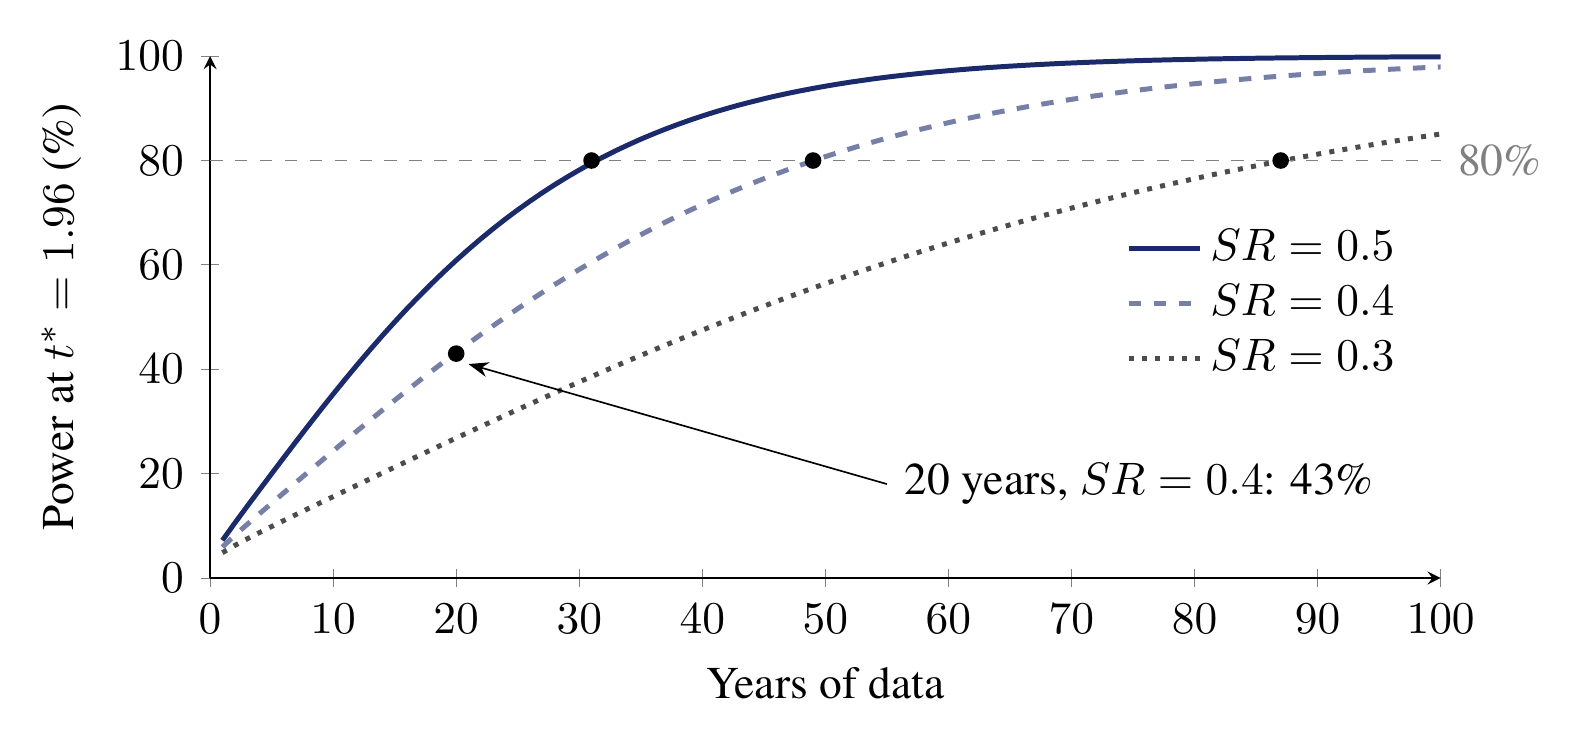
\includegraphics[width=0.85\linewidth]{images/fig25-1-power.png}
\caption{Power to detect a true Sharpe ratio at $t^* = 1.96$, by years of data. Reaching 80\% power takes 31 years at a Sharpe ratio of 0.5, 49 years at 0.4 and 87 years at 0.3. With 20 years, a real Sharpe ratio of 0.4 is detected only 43\% of the time.}
\label{fig:25-power}
\end{figure}

\textbf{Multiple testing.} Testing $N$ independent hypotheses at 5\% each produces about $0.05N$ false positives. The \textbf{Bonferroni} correction tests each at $\alpha/N$, which raises the required t-statistic: about 2.81 for 10 tests and 3.48 for 100, two-sided (Figure~\ref{fig:25-bonf}). Chapter 4 covers less conservative alternatives.

\begin{figure}[htbp]
\centering
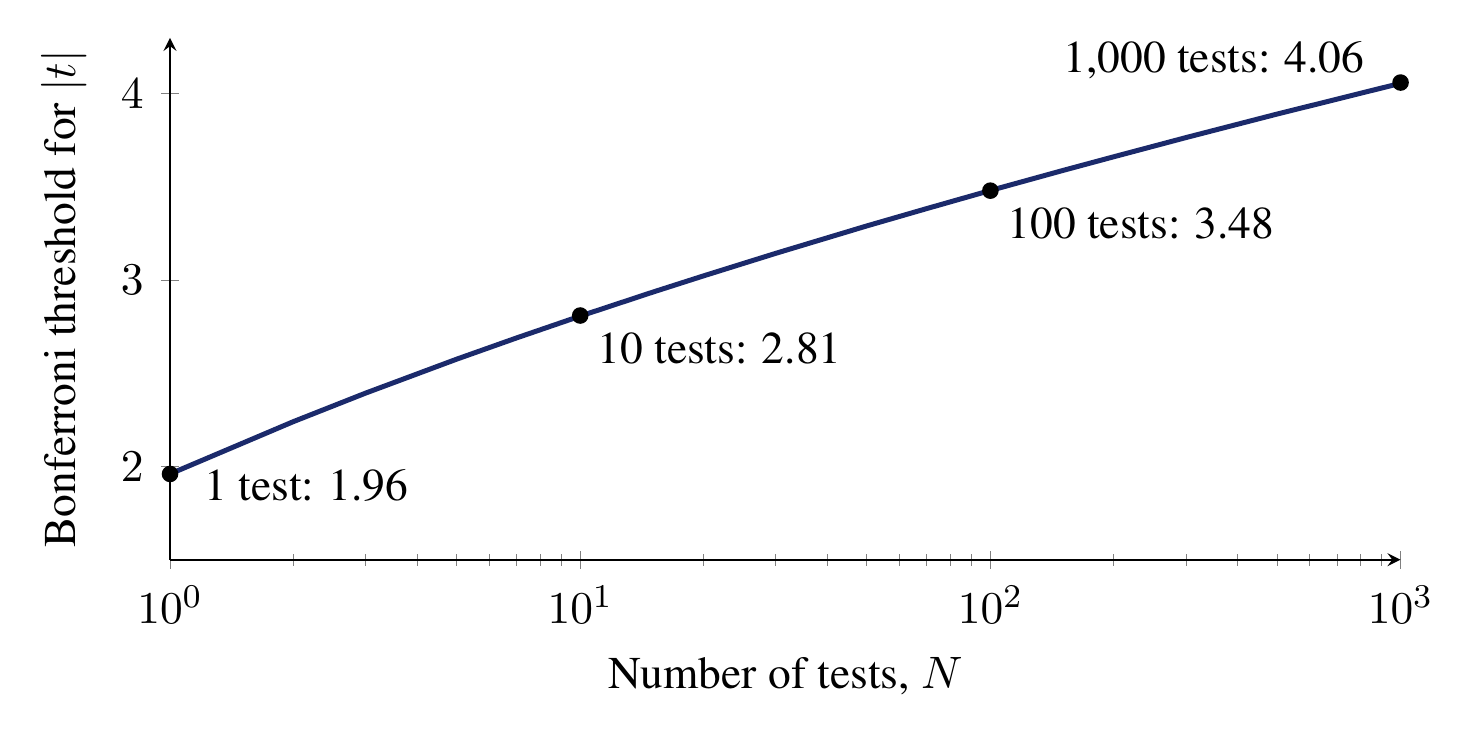
\includegraphics[width=0.85\linewidth]{images/fig25-2-bonferroni.png}
\caption{The Bonferroni threshold for a two-sided test at a 5\% family-wise level, as the number of tests grows. It rises from 1.96 for one test to 2.81 for 10, 3.48 for 100 and 4.06 for 1,000.}
\label{fig:25-bonf}
\end{figure}

\textbf{Bayesianized p-values.} Harvey (2017) proposed combining a test result with prior odds. The \textbf{minimum Bayes factor} is the most a result can favour the alternative:
\begin{equation}
  \mathrm{MBF} = \exp\!\left(-\frac{t^2}{2}\right)
  \label{eq:25-mbf}
\end{equation}
Multiplied by the prior odds against an effect, it bounds the probability that the null is still true. With a t-statistic of 1.96 and prior odds of 4 to 1 against, that probability is at least 37\%.

\textbf{Identification and causal inference.} Many finance claims are causal: a policy, an event or a characteristic \emph{causes} a change in returns or behavior. Angrist and Pischke (2009) frame identification as finding variation that is as good as randomly assigned, and they describe the main tools:

\begin{itemize}
  \item \textbf{randomized experiments};
  \item \textbf{differences-in-differences}, which compare the change in a treated group with the change in a control group;
  \item \textbf{instrumental variables}, which use a source of variation that affects the outcome only through the variable of interest;
  \item \textbf{regression discontinuity}, which compares units just above and just below a threshold.
\end{itemize}

In asset pricing, most claims are predictive rather than causal (a characteristic predicts returns), and the main threats are data mining and look-ahead. In corporate finance and household finance, the main threat is \textbf{confounding}: the variable of interest moves with something else that drives the outcome.

\textbf{Further reading.} Angrist and Pischke, \emph{Mostly Harmless Econometrics}, and Cunningham, \emph{Causal Inference: The Mixtape} (causal inference and research design); Wasserman, \emph{All of Statistics} (hypothesis testing and power); Harvey, ``The Scientific Outlook in Financial Economics'' (\emph{Journal of Finance}, 2017); Nosek and others, ``The Preregistration Revolution'' (\emph{PNAS}, 2018).

\section{Turning a claim into testable hypotheses}
\label{sec:25-hypotheses}

Claims in finance usually arrive in loose language: ``value beats growth'', ``momentum works'', ``AI can read the news''. A testable version needs five elements:

\begin{enumerate}
  \item \textbf{The object.} What exactly earns what? For example, the value-weighted top decile of stocks by book-to-market minus the bottom decile, with NYSE breakpoints.
  \item \textbf{The quantity.} Mean return, alpha against a model, Sharpe ratio, out-of-sample $R^2$ or a regression slope.
  \item \textbf{The comparison.} Against zero, a benchmark or another method.
  \item \textbf{The direction.} Most claims are one-sided: the effect is positive, or the new method is better.
  \item \textbf{The decision rule.} What result counts as support, what as failure and what as inconclusive.
\end{enumerate}

Each claim chapter in this book started from a sentence (``The claim'') and turned it into tests in the lab. The same discipline applies to new research. Write the claim as one falsifiable sentence, then translate it into a \textbf{primary hypothesis}, the single test that decides the question, and a short list of \textbf{secondary hypotheses}, which add depth but cannot rescue a failed primary test.

The decision rule matters as much as the test. ``Support'' should require more than statistical significance: a sign and size consistent with the claim, and significance in the sample the claim is about (often the period after publication). ``Failure'' should be defined too, so that a null result is reported as evidence rather than as a disappointment.

\section{Sample, benchmarks and controls}
\label{sec:25-sample}

\textbf{Sample.} The sample should be chosen for reasons that do not depend on the result:

\begin{itemize}
  \item \textbf{Period.} The full available history, the period after the original publication (for replications), or both.
  \item \textbf{Universe.} Which securities are included, and how microcaps are treated. Hou, Xue and Zhang (2020) found that about 65\% of 452 anomalies were insignificant at the 5\% level once microcaps were limited by NYSE breakpoints and value weighting. Chen and Zimmermann (2022), using the original papers' own methods, reproduced nearly all clearly significant predictors. Much of the difference between the two studies lies in such design choices.
  \item \textbf{Data vintage.} Data are revised. Record the download date and keep a copy.
  \item \textbf{Exclusions.} State them in advance: financial firms, low-priced stocks, missing data.
\end{itemize}

\textbf{Benchmarks.} A claim that a method is ``better'' needs a strong benchmark, not a straw man:

\begin{itemize}
  \item the historical mean for return forecasts (Chapters 5 and 7);
  \item 1/N for portfolios (Chapter 19);
  \item AR and HAR models for forecasting series (Chapters 11 and 22);
  \item a linear model with the same inputs for machine learning (Chapter 21);
  \item a finance dictionary for language models (Chapter 23).
\end{itemize}

\textbf{Controls.} For return claims, control for known factors (market, size, value, momentum, profitability, investment) and report alphas. For causal claims, choose controls that block confounding paths without introducing new bias; Angrist and Pischke warn against ``bad controls'' that are themselves outcomes of the treatment.

\textbf{Out of sample.} Reserve data that will be used only once, for the final test. Chapter 5 covers walk-forward designs, purging and embargoes.

\section{Power: how much data is enough}
\label{sec:25-power}

Most finance effects are small relative to the noise in returns, and samples are short. Power analysis answers two questions before a study begins: whether the sample could detect the effect if it exists, and what a non-significant result would mean.

\begin{center}
\small
\begin{tabularx}{0.9\linewidth}{@{}>{\raggedright\arraybackslash}p{0.17\linewidth}>{\raggedright\arraybackslash}X>{\raggedright\arraybackslash}X>{\raggedright\arraybackslash}X@{}}
\toprule
True Sharpe ratio & Years for 80\% power at $t = 1.96$ & Years for 80\% power at $t = 3.0$ & Power with 20 years at $t = 1.96$ \\
\midrule
0.2 & 196 & 369 & 14\% \\
0.3 & 87 & 164 & 27\% \\
0.4 & 49 & 92 & 43\% \\
0.5 & 31 & 59 & 61\% \\
0.75 & 14 & 26 & 92\% \\
1.0 & 8 & 15 & 99\% \\
\bottomrule
\end{tabularx}
\end{center}

The table, computed in Lab 25, makes three points:

\begin{itemize}
  \item \textbf{Many claims cannot be settled with the data available.} A factor with a true Sharpe ratio of 0.3, typical of published anomalies after publication, needs almost 90 years of data for a reliable test at $t = 1.96$, and more than 160 at $t = 3$.
  \item \textbf{Short-sample results are mostly noise.} With 20 years of data, a real effect with a Sharpe ratio of 0.3 is detected only about a quarter of the time. A backtest with a high Sharpe ratio over a short period is more likely to reflect luck than skill.
  \item \textbf{Absence of evidence is weak evidence of absence.} A non-significant result from an underpowered study says little. Report the power alongside the result, or report a confidence interval, which shows the range of effects the data cannot rule out.
\end{itemize}

The formulas assume normal, independent returns. Lab 25 checks them by simulation with fat tails and autocorrelation, which change the rejection rates of naive t-tests. That is one more reason to use robust standard errors (Chapter 3).

For predictive regressions the requirements are similar. A monthly $R^2$ of 0.5\% needs about 1,560 months, 130 years, for 80\% power at $t = 1.96$. Because hundreds of ideas have been tested on the same data, the relevant threshold is higher than 1.96: the Bonferroni threshold for 100 tests is about 3.5.

\section{Pre-registration}
\label{sec:25-prereg}

A \textbf{pre-registration} is a written, time-stamped plan made before the researcher sees the results. It separates \textbf{confirmatory} analysis, planned in advance, from \textbf{exploratory} analysis, discovered along the way. Both are valuable, but only the first supports the usual interpretation of a p-value.

A pre-registration for a finance study covers:

\begin{enumerate}
  \item \textbf{The claim}, in one sentence.
  \item \textbf{Hypotheses}: the primary hypothesis and its direction, and the secondary hypotheses.
  \item \textbf{Data}: sources, vintage and how they will be obtained.
  \item \textbf{Sample and exclusions}, fixed in advance.
  \item \textbf{The primary test}: statistic, standard errors and threshold.
  \item \textbf{Secondary tests and the robustness grid.}
  \item \textbf{Power}: the expected effect size, the sample and the resulting power.
  \item \textbf{Decision rules}: what counts as support, failure or an inconclusive result.
  \item \textbf{Reporting}: what will be reported whatever the outcome.
  \item \textbf{Deviations}: a commitment to list and justify any departure from the plan.
\end{enumerate}

The plan must be fixed in a way others can verify. A commit to a public repository, a post on the Open Science Framework or a hash of the document published somewhere time-stamped all work. Lab 25 writes the document and appends its \textbf{SHA-256 hash}, a fingerprint that changes if a single character changes, so that any later edit is detectable.

\textbf{The problem of old data.} Pre-registration is cleanest when the data do not yet exist. In finance, most data are historical and may already have been seen. Three partial remedies help:

\begin{itemize}
  \item pre-register a test on the period after the original study, which is the logic of post-publication tests throughout this book;
  \item pre-register on data that will arrive in the future, such as the next five years of returns;
  \item hold out data the researcher commits not to examine, such as an international sample.
\end{itemize}

\textbf{Registered reports.} Some journals review the plan rather than the results, and accept the paper in principle before the data are analyzed. The \emph{Journal of Accounting Research} ran its 2017 conference this way: authors pre-registered their analyses and received provisional acceptance regardless of outcome. Registered reports remove the incentive to find a significant result, because publication no longer depends on one.

\section{Robustness grids and reporting null results}
\label{sec:25-robust}

Every empirical study involves choices that are individually reasonable: the sample start, the breakpoints, the weighting, the treatment of outliers, the holding period. Gelman and Loken (2014) called the result a ``garden of forking paths'': even a researcher who runs only one analysis may have chosen it after seeing the data, and the reported p-value no longer means what it says.

Lab 25 makes the problem concrete. A signal that is pure noise is tested in 36 reasonable ways (three sample starts, three portfolio cuts, two weightings, two treatments of January), 300 times over. The pre-chosen specification is significant in about 4\% of studies, close to the nominal 5\%. At least one of the 36 specifications is significant in about 39\%. A researcher who reports the best of 36 has close to a two-in-five chance of a false discovery.

The remedy is to report the whole grid, not only the preferred specification:

\begin{itemize}
  \item A \textbf{specification curve} (Simonsohn, Simmons and Nelson 2020) plots the estimate for every reasonable specification, sorted by size, with the choices shown underneath. Lab 25 draws one for the size effect across 36 specifications.
  \item Report the share of specifications that are significant and the range of estimates, and say which specification was pre-registered as primary.
  \item If results depend on one choice, say so and explain why that choice is right.
\end{itemize}

\textbf{Null results.} A well-designed test that finds no effect is a result. It should be reported with its power and confidence interval, so readers can see which effect sizes it rules out. \textbf{Publication bias}, the tendency for significant results to be published and null results to be filed away, distorts the literature (Chapter 10). Harvey (2017) noted how few published t-statistics fall below 2. Replication-friendly outlets, discussed in Chapter 26, publish well-designed null results.

\section{Reading finance papers critically}
\label{sec:25-reading}

The same checklist that guides a study also helps in reading one. Before accepting a paper's conclusion, ask:

\begin{enumerate}
  \item \textbf{The claim.} Is it stated precisely enough to be false? What is the primary test?
  \item \textbf{Prior plausibility.} Is there an economic reason for the effect, a risk or a behavioral bias, stated before the evidence?
  \item \textbf{Sample.} Why this period and universe? Does the result hold after the original publication, in other countries, and without microcaps?
  \item \textbf{Benchmarks and controls.} Is the comparison with a strong benchmark? Are known factors controlled for?
  \item \textbf{Statistics.} Are standard errors robust to autocorrelation and heteroskedasticity? Is the t-statistic adjusted for the number of tests the authors and the field have run?
  \item \textbf{Power and size.} Is the sample long enough? Is the effect economically meaningful, not just statistically significant?
  \item \textbf{Forking paths.} How many specifications are shown? Do the results survive reasonable alternatives?
  \item \textbf{Implementation.} Are trading costs, capacity and data availability at the time accounted for?
  \item \textbf{Look-ahead.} Could any input have been known only later, including through a pre-trained model?
  \item \textbf{Replication.} Are data and code available? Has anyone replicated it?
\end{enumerate}

The disagreement between Hou, Xue and Zhang (2020) and Chen and Zimmermann (2022) shows why the details matter. Both studies examined the same anomaly literature. One found that most anomalies failed and the other that nearly all clearly significant predictors replicated, largely because they made different, defensible choices about microcaps, weighting and breakpoints. Jensen, Kelly and Pedersen (2023) argued, using a Bayesian framework and data from 93 countries, that most factors do replicate. A careful reader asks which choices drive a result and whether the claim survives the alternatives.

\section{Lab 25: pre-registration and power analysis}
\label{sec:25-lab}

\begin{callout}
\textbf{Lab 25 at a glance.} \emph{Question:} how much data does a claim need, how many false discoveries do forking paths create, and how is a plan frozen before the test? \emph{Data:} Portfolios Formed on Size from the Kenneth R. French Data Library, for Part C; the other parts need no market data. \emph{Code:} runs as a script (\texttt{python lab25.py}, or \texttt{python lab25.py -{}-claim-file my\_claim.json -{}-expected-sharpe 0.4} for your own claim) or as a notebook (\texttt{lab25\_walkthrough.ipynb}), using the design tools of the book's \texttt{fintest} module.
\end{callout}

The lab has five parts:

\begin{itemize}
  \item \textbf{Part A, power for returns.} It computes the years of data needed to detect Sharpe ratios from 0.2 to 1.0 at $t = 1.96$ and $t = 3.0$, and checks the formula by simulation, first with normal returns and then with fat tails (Student-$t$ with 4 degrees of freedom) and autocorrelation of 0.15 (Figure 25.3).
  \item \textbf{Part B, predictability and multiple testing.} It computes the months needed to detect an $R^2$ from 0.2\% to 10\%, and the Bonferroni t-threshold as the number of tests grows from 1 to 1,000 (Figure 25.4).
  \item \textbf{Part C, forking paths.} It draws a specification curve for the size effect, smallest minus largest size portfolio, across 36 combinations of research choices (Figure 25.5). It also tests a pure-noise signal in the same 36 ways, 300 times (Figure 25.6).
  \item \textbf{Part D, Bayesianized p-values.} It tabulates the lowest probability that the null is true for t-statistics from 1.96 to 4 and prior odds from 1:1 to 99:1 against (Figure 25.7).
  \item \textbf{Part E, pre-registration.} It writes \texttt{preregistration.md} for the size effect as an example, or for the reader's own claim supplied as a JSON file, with the power analysis filled in and a SHA-256 hash appended.
\end{itemize}

\textbf{What the run shows.} Parts A, B, D and E do not depend on market data, and their results are exact or simulated by design. Part C was run with simulated size portfolios.

\begin{itemize}
  \item The power table is the one shown in Section~\ref{sec:25-power}. Simulation confirmed about 80\% power at the computed sample sizes with normal returns. With fat tails and autocorrelation, the naive t-test's rejection rate fell to 76\% to 78\%.
  \item The pure-noise signal was significant in 4.0\% of studies in the pre-chosen specification and in 38.7\% somewhere among the 36 specifications.
  \item In the simulated size portfolios, the 36 estimates of the size effect ranged from $-2.1\%$ to $+5.3\%$ a year, and 10 of the 36 were significant. Which result a researcher reported would depend on which path they took.
  \item At $t = 1.96$, the lowest probability that the null is true was 13\% with even prior odds, 37\% with odds of 4:1 against and 57\% with odds of 9:1 against.
\end{itemize}

\section{The reporting checklist}
\label{sec:25-checklist}

This checklist is for empirical finance papers, dissertation chapters and replication reports. Each item should be answerable from the text.

\textbf{Claim and plan}

\begin{itemize}
  \item[$\square$] The claim is stated as one falsifiable sentence.
  \item[$\square$] The primary hypothesis, its direction and the decision rule are stated.
  \item[$\square$] A pre-registration exists, with its date and location, or the absence of one is acknowledged.
  \item[$\square$] Deviations from the plan are listed and justified.
\end{itemize}

\textbf{Data and sample}

\begin{itemize}
  \item[$\square$] Sources, download dates and versions are given.
  \item[$\square$] The sample period, universe and exclusions are stated and justified.
  \item[$\square$] Every variable was available at the time it is used.
\end{itemize}

\textbf{Tests}

\begin{itemize}
  \item[$\square$] The benchmark is the strongest reasonable one.
  \item[$\square$] Standard errors are robust to autocorrelation and heteroskedasticity, and the method is named.
  \item[$\square$] The number of tests run is reported, and thresholds are adjusted where appropriate.
  \item[$\square$] Power is reported for the primary test.
\end{itemize}

\textbf{Results}

\begin{itemize}
  \item[$\square$] Effect sizes are reported in economic units (percent a year, basis points), with confidence intervals.
  \item[$\square$] The full robustness grid or specification curve is shown.
  \item[$\square$] Results after trading costs are reported where the claim is about returns an investor could earn.
  \item[$\square$] Out-of-sample or post-publication results are reported separately.
  \item[$\square$] Null and contrary results are reported.
\end{itemize}

\textbf{Transparency}

\begin{itemize}
  \item[$\square$] Code and data (or instructions to obtain them) are publicly available.
  \item[$\square$] The conclusion is dated and states what new evidence would change it.
\end{itemize}

\section*{Exercises}
\addcontentsline{toc}{section}{Exercises}

\subsection*{Conceptual (all readers)}

\begin{enumerate}
  \item A strategy's true Sharpe ratio is 0.25. How many years of data are needed for 80\% power at $t = 1.96$? What is the power with 30 years?
  \item A researcher tests 20 independent signals and reports the one with $t = 2.6$. Is it significant at the 5\% family-wise level under Bonferroni?
  \item With prior odds of 9 to 1 against a new anomaly, what t-statistic is needed for the lowest probability of the null to fall below 10\%?
  \item Rewrite the claim ``low-volatility stocks are a free lunch'' as a primary hypothesis with a decision rule.
\end{enumerate}

\subsection*{Lab extensions (technical readers)}

\begin{enumerate}
  \setcounter{enumi}{4}
  \item Part C: run on real data. How many of the 36 size-effect specifications are significant? Which choices matter most?
  \item Extend the noise experiment to 72 specifications by adding a holding-period choice. What share of studies now finds a significant result somewhere?
  \item {\sloppy Write a pre-registration for a claim from Chapters 7 to 24, using \texttt{-{}-claim-file}. Commit it to a public repository before running the test.\par}
  \item Compare the analytic power with the simulated power for a Sharpe ratio of 0.5 when returns have autocorrelation of 0.3. Why does the naive t-test misbehave?
\end{enumerate}

\subsection*{Projects}

\begin{enumerate}
  \setcounter{enumi}{8}
  \item Choose a published finance paper. Apply the checklist in Section~\ref{sec:25-reading} and write a one-page assessment.
  \item Design a study of a causal claim from corporate or household finance, such as the effect of a change in disclosure rules on trading costs. Which identification strategy would you use, and what would threaten it?
\end{enumerate}

\section*{References}
\addcontentsline{toc}{section}{References}

\begin{itemize}
  \item Angrist, J. D. and Pischke, J.-S. (2009). \emph{Mostly Harmless Econometrics: An Empiricist's Companion}. Princeton: Princeton University Press.
  \item Chen, A. Y. and Zimmermann, T. (2022). Open Source Cross-Sectional Asset Pricing. \emph{Critical Finance Review} 11(2): 207--264.
  \item Gelman, A. and Loken, E. (2014). The Statistical Crisis in Science. \emph{American Scientist} 102(6): 460--465.
  \item Harvey, C. R. (2017). Presidential Address: The Scientific Outlook in Financial Economics. \emph{Journal of Finance} 72(4): 1399--1440.
  \item Harvey, C. R., Liu, Y. and Zhu, H. (2016). \ldots and the Cross-Section of Expected Returns. \emph{Review of Financial Studies} 29(1): 5--68.
  \item Hou, K., Xue, C. and Zhang, L. (2020). Replicating Anomalies. \emph{Review of Financial Studies} 33(5): 2019--2133.
  \item Jensen, T. I., Kelly, B. and Pedersen, L. H. (2023). Is There a Replication Crisis in Finance? \emph{Journal of Finance} 78(5): 2465--2518.
  \item Nosek, B. A., Ebersole, C. R., DeHaven, A. C. and Mellor, D. T. (2018). The Preregistration Revolution. \emph{Proceedings of the National Academy of Sciences} 115(11): 2600--2606.
  \item Simonsohn, U., Simmons, J. P. and Nelson, L. D. (2020). Specification Curve Analysis. \emph{Nature Human Behaviour} 4(11): 1208--1214.
\end{itemize}

\textbf{Data:} Kenneth R. French Data Library: Portfolios Formed on Size.
